\documentclass[class=book, crop=false, oneside, 12pt]{standalone}
\usepackage{standalone}
\usepackage{../../style}
\usepackage[normalem]{ulem}
\graphicspath{{./assets/images/}}

% arara: pdflatex: { synctex: yes, shell: yes }
% arara: latexmk: { clean: partial }
\begin{document}
\chapter{Esami}
\section{Prototipo di test di LFC, 2021}

%dovremmo in qualche modo inserire di bruttanza il testo della prova perchè non ho la minima voglia di ricopiare le parti iniziali quando possiamo rubarle

Benvenuti in questa meravigliosa sezione dove avremo modo di affrontare assieme l'esame fornito dalla Prof.ssa Quaglia per potersi preparare al meglio alla prova vera e propria. Cominciamo col dire che per affrontare tale esame è necessario:

\begin{enumerate}
    \item avere ben chiaro quanto fatto fino ad ora: gli esercizi proposti spaziano dalle derivazioni leftmost trattate all'inizio del corso fino alle regole degli SDD; assicuratevi quindi di essere ben preparati.
    \item trovare la strada più breve: il procedimento algoritmico sarà sempre a vostra disposizione avendo studiato, ma è pur sempre lungo. Arrivare al DFA minimo passando per Thompson, la Subset Construction e la Minimizzazione vi porterà via un sacco di tempo: all'esame avrete un'ora e mezza per cui cercate di perdere meno tempo possibile.
    \item saper spaziare: soprattutto nell'ultimo esercizio verrà richiesto di avere fantasia e saper applicare quanto studiato in maniera differente dal semplice ragionamento.
\end{enumerate}

Detto questo, cominciamo.

\subsection{Esercizio 1}

Se \(\{ww \mid w \in \L((a \mid b)^*)\}\) è un linguaggio regolare rispondere “SI”, altrimenti rispondere “NO”.

Analizziamo il tutto a mente fredda: la domanda è se il linguaggio proposto è regolare, una sottoclasse dei linguaggi liberi. In questo caso non ha senso perdersi sulla definizione in quanto il linguaggio di partenza (i.e. quello a cui appartiene w) è sicuramente regolare in quanto è denotato da un'espressione regolare. A questo sembrerebbe che la risposta sia a portata di mano: “Visto che i linguaggi regolari sono chiusi rispetto alla concatenazione allora il linguaggio fornito è regolare”, giusto? NO! 

Osserviamo meglio il tutto: se veramente valesse la proprietà di concatenazione potremmo scrivere il tutto come 

\begin{align*}
    \L = \{w_1 w_2 \mid w_1 \in \L_1 \land w_2 \in \L_2\}
\end{align*}

dove \(L_1\) e \(L_2\) sono due linguaggi regolari. 

Se questo fosse vero vorrebbe dire che \(\L_1 = \L_2 = \L((a \mid b)^*)\) e quindi che \(w' = ab \in \{w_1 w_2 \mid w_1 \in \L((a \mid b)^*) \land w_2 \in \L((a \mid b)^*)\}\), tuttavia \(w' \notin \{ww \mid w \in \L((a \mid b)^*)\}\): non possiamo dunque sfruttare tale proprietà a nostro vantaggio.

L'ultima spiaggia è dunque utilizzare il \emph{Pumpin Lemma} per poter arrivare ad una conclusione:

\begin{itemize}
    \item Supponiamo che \(\L = \{ww \mid w \in L((a \mid b)^*)\}\) sia un linguaggio regolare
    \item Prendiamo \(p\) intero positivo arbitrario 
    \item Costruiamo la parola \(z = a^pb^pa^pb^p\) (con \(w = a^pb^p \in \L\)); \(\mid z \mid > p\)
    \item \(\forall u, v, w \textrm{ se } (z = uvw \textrm{ e } \mid uv \mid \; \leq p \textrm{ e } \mid v \mid \; > 0) \Rightarrow (\exists i \in N : uv^iw \notin \L)\)
\end{itemize}

Dovrebbe essere infatti abbastanza facile osservare che in questo caso, per non sbilanciare la stringa, dovrebbe essere necessario poter modificare contemporaneamente due porzioni che si trovano a distanza maggiore di \(p\). 

Dunque tale linguaggio non è regolare e la risposta corretta è \textbf{“NO”}. Visto che non è richiesta alcuna dimostrazione un modo per potersi accorgere di ciò è immaginare un NFA o DFA che rappresenti il linguaggio: ciò è impossibile perchè dovrebbe memorizzare il valore di \(w\) per poi ripeterlo. Questo vorrebbe dire creare infiniti stati per cui, letta una parola, l'automa obblighi a crearne una identica di seguito. 

\subsection{Esercizio 2}

Se la seguente affermazione è vera rispondere “VERO”, altrimenti rispondere “FALSO”: “Se i linguaggi \(\L_1 \textrm{ e } \L_2\) sono entrambi regolari allora \(\L_1 \cup \L_2\) è regolare.”

In questo caso per rispondere è sufficiente accorgersi del fatto che l'affermazione corrisponde alla \emph{proprietà di chiusura dei linguaggi regolari rispetto all'unione}: infatti, dati \(\L_1 \textrm{ e } \L_2\) linguaggi regolari, si ha che 

\begin{align*}
    \L = \{w \mid w \in \L_1 \lor w \in \L_2\}
\end{align*}

e quindi \(\L\) è ancora un linguaggio regolare. 

La risposta all'esercizio è dunque \textbf{“VERO”}.

\subsection{Esercizio 3}

Sia \(r=b^* \mid b^* a (\epsilon \mid a \mid b)^*\)e sia \(\mathcal{D}\) il DFA minimo per il riconoscimento di \(\L(r)\). Dire quanti stati ha \(\mathcal{D}\) e quanti di questi stati sono finali.

Per poter risolvere l'esercizio è possibile applicare la Thompson's Construction per ottenere un NFA, successivamente la Subset Construction per trasformarlo in un DFA ed infine la DFA Minimization per ottenere \(\mathcal{D}\). Il procedimento, seppur efficacie, è troppo lungo da svolgere (i.e. o saltate l'esercizio e ci ritornate dopo oppure trovate un metodo furbo per farlo): per questo motivo è meglio osservare direttamente la regex. Il linguaggio denotato è \(\{b^k \mid k \geq 0\} \cup \{b^i a a^j b^k \mid i \geq 0, j \geq 0, k \geq 0\}\): se riuscissimo a trovare un DFA che ci permette di ottenere questo linguaggio poi potremmo ridurlo. 

Partiamo dal primo caso: vogliamo avere la possibilità di generare 0 o più ripetizioni di \(b\), dunque abbiamo bisogno che lo stato iniziale sia anche lo stato finale (in questo modo si ha la possibilità di ottenere la stringa vuota) e che vi sia un self-loop con etichetta \(b\) (per poter considerare le parole del tipo \(b^k\)).

\begin{figure}[H]
	\centering
    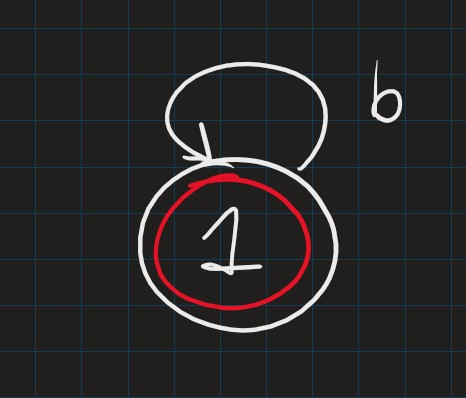
\includegraphics[width=.3\textwidth]{dfa-pt1-ex3.jpg}
    \caption{Es 1: DFA Parziale \(b^*\)}
    \label{fig:dfa-pt1-ex3}
\end{figure}

Passiamo ora al secondo insieme di parole riconosciute: essendo che la prima parte è identica possiamo riciclare lo stato creato precedentemente, con la differenza che in questo caso non dovrà essere terminale; infatti dobbiamo avere almeno un'occorrenza di \(a\). Proprio per questo motivo aggiungiamo un arco con etichetta \(a\) che porta in un nuovo stato terminale. A questo punto non ci resta che gestire il caso delle 0 o più occorrenze di \(a\) e di \(b\): per fare ciò basterà come visto precedentemente aggiungere un self-loop per ognuno dei terminali che devono essere ripetuti.


\begin{figure}[H]
	\centering
    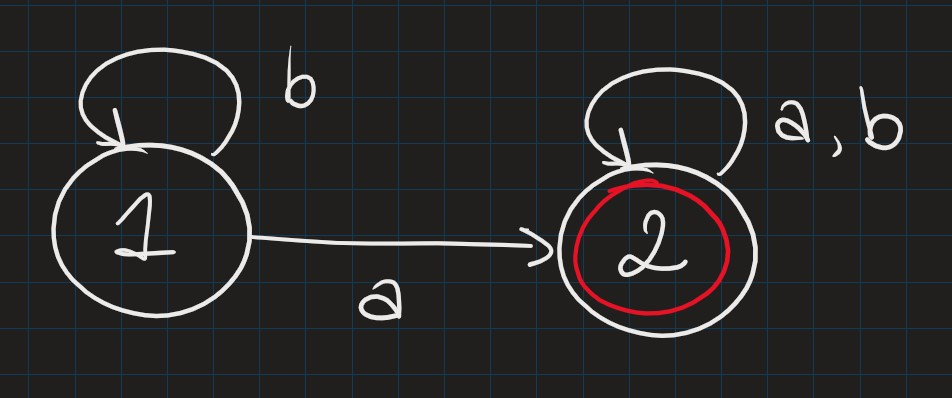
\includegraphics[width=.6\textwidth]{dfa-pt2-ex3.jpg}
    \caption{Es 1: DFA Parziale \(b^* a (\epsilon \mid a \mid b)^*\)}
    \label{fig:dfa-pt2-ex3}
\end{figure}

A questo punto abbiamo quasi concluso, la cosa che ci manca è unificare questi due DFA in modo che ci diano la possibilità di scegliere fra le due tipologie di parole denotate dalla nostra espressione regolare. Ancora una volta, una tecnica potrebbe essere quella di applicare l'operazione di unione prevista dalla Thompson's Construction e procedere come citato all'inizio. In questo caso però basta osservare che, per poter considerare valide anche le parole del tipo \(\{b^k \mid k \geq 0\}\), basta semplicemente considerare lo stato 1 del secondo automa come terminale: 

\begin{figure}[H]
	\centering
    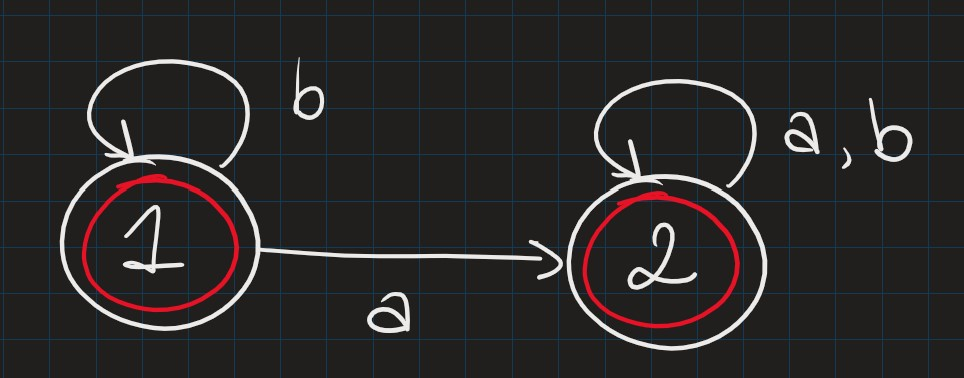
\includegraphics[width=.6\textwidth]{dfa-pt3-ex3.jpg}
    \caption{Es 1: DFA Parziale \(b^* \mid b^* a (\epsilon \mid a \mid b)^*\)}
    \label{fig:dfa-pt3-ex3}
\end{figure}

A questo punto possiamo applicare la minimizzazione del DFA:

\begin{itemize}
    \item Separiamo gli stati terminali da quelli non terminali ottenendo \(B_1 = \emptyset\) e  \(B_2 = \{1, 2\}\)
    \item Visto che \(B_2\) contiene la totalità degli stati che costituiscono il DFA, non è possibile che vi siano archi che vadano in altri stati al di fuori di \(B_2\)
    \item Il DFA minimo è costituito dunque da \(B_2\)
\end{itemize}

Il DFA minimizzato \(\mathcal{D}\) è dunque così costruito:

\begin{figure}[H]
	\centering
    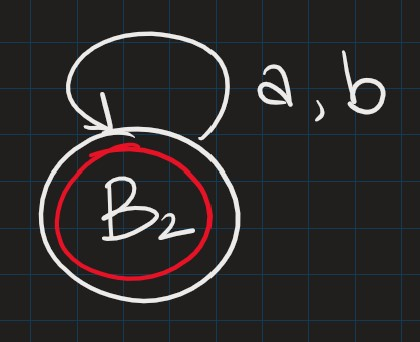
\includegraphics[width=.3\textwidth]{dfa-minimized-ex3.jpg}
    \caption{Es 1: DFA Minimizzato \(b^* \mid b^* a (\epsilon \mid a \mid b)^*\)}
    \label{fig:dfa-minimized-ex3}
\end{figure}

\(\mathcal{D}\) possiede dunque \textbf{1 stato} e \textbf{1 stato finale}

\subsection{Esercizio 4}

Chiamiamo \(\mathcal{D}\) il DFA ottenuto da \(\mathcal{N}_1\) per subset construction e \(Q_l\) lo stato iniziale di \(\mathcal{D}\).  Dire a quale sottoinsieme degli stati di \(\mathcal{N}_1\) corrisponde \(Q[ab]\).

Per maggiore chiarezza possiamo rappresentare l'automa per intero:

\begin{figure}[H]
	\centering
    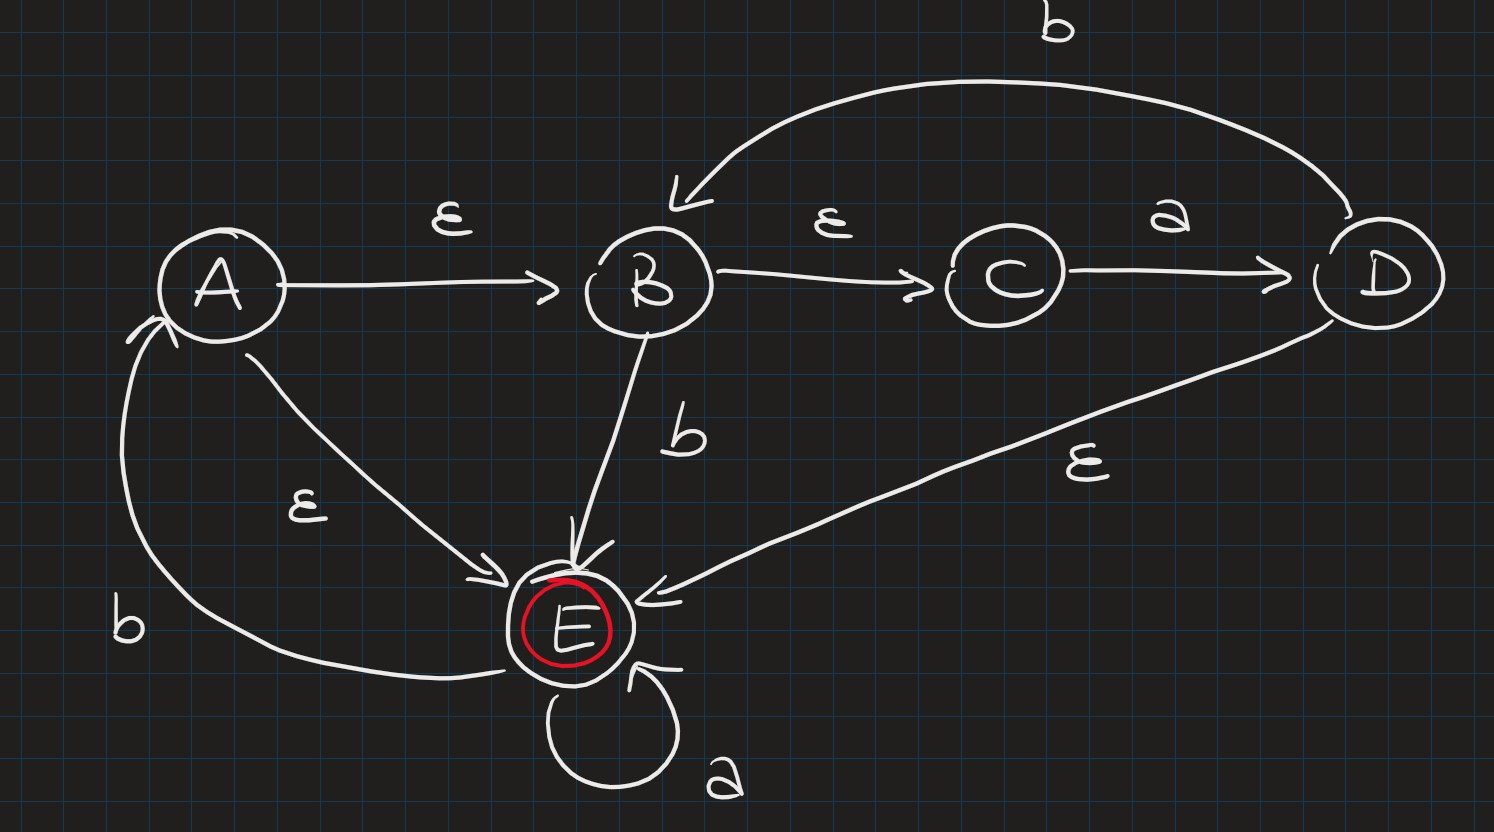
\includegraphics[width=.8\textwidth]{nfa-ex4.jpg}
    \caption{Es 1: NFA di partenza}
    \label{fig:nfa-ex4}
\end{figure}

Eseguiamo dunque la Subset Construction:

\begin{table}[H]
    \centering
    \subimport{assets/tables/}{subset-construction-ex4.tex}
    \caption{Es 4: Subset Construction}
    \label{tab:subset-construction-ex4}
\end{table}

\(\mathcal{D}\) risulta dunque così costruito:

\begin{figure}[H]
	\centering
    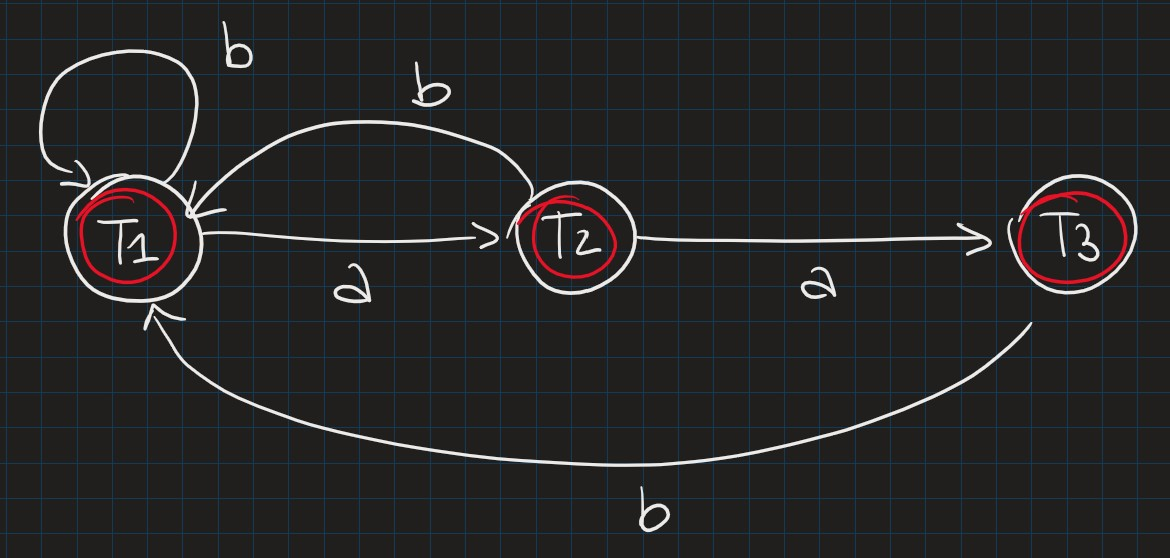
\includegraphics[width=.8\textwidth]{sc-ex4.jpg}
    \caption{Es 1: DFA risultante dalla Subset Construction}
    \label{fig:sc-ex4}
\end{figure}

A questo punto, partendo dallo stato iniziale \(T_1\), è possibile spostarsi allo stato indicato seguendo il percorso \(ab\): lo stato di destinazione è dunque lo stato \(T_1\), quindi la risposta è corretta è \textbf{\{A, B, C, E\}}

\subsection{Esercizio 5}

Chiamiamo \(\mathcal{D}_m\) il  DFA  ottenuto  per  minimizzazione  di \(\mathcal{D}_1\) e \(P_1\) o  stato  iniziale  di \(\mathcal{D}_m\). Dire a quale sottoinsieme degli stati di \(\mathcal{D}_1\) corrisponde \(P[abab]\)

L'esercizio proposto è identico a quello svolto durante una lezione del corso: la sua risoluzione si può trovare in ~\ref{subsec:dfa-minimization} \emph{Esercizi sulla minimizzazione DFA, Esercizio 2}.

\subsection{Esercizio 6}

Scrivere l’intera riga della tabella di parsing \(LL(1)\) per \(\G_1\) relativa al non-terminale \(B\).

Riportiamo \(\G_1\) per praticità

\begin{align*}
    S &\to AaB \mid b \\
    A &\to BcBaA \mid \epsilon \\
    B &\to \epsilon
\end{align*}

Per poter calcolare la tabella di parsing \(LL(1)\) è necessario computare innanzitutto first e follow per ogni driver della grammatica \(\G_1\).

\begin{table}[H]
    \centering
    \subimport{assets/tables/}{first-follow-ex6.tex}
    \caption{Es 6: First e Follow \(\G_1\)}
    \label{tab:first-follow-ex6}
\end{table}

A questo punto è possibile applicare l'algoritmo per la computazione della parsing table \(LL(1)\): visto che ci interessa solamente la riga relativa al non-terminale \(B\) concentriamoci solamente sulla produzione \(B \to epsilon\)

\begin{itemize}
    \item \(\forall b \in first(B) \setminus \epsilon, \textrm{ add } B \to epsilon \textrm{ to } M[B, b]\) (che non comporta nessuna modifica nella tabella)
    \item Visto che \(\epsilon \in first(B)\), allora \(\forall x \in follow(B), \textrm{ add } B \to epsilon \textrm{ to } M[B, x]\)
\end{itemize}

La riga identificata dal non-terminale \(B\), nonché soluzione dell'esercizio, sarà dunque così rappresentata:

\begin{table}[H]
    \centering
    \subimport{assets/tables/}{parsing-table-ll1-ex6.tex}
    \caption{Es 6: Riga Parsing Table \(LL(1)\)}
    \label{tab:parsing-table-ll1-ex6}
\end{table}

\subsection{Esercizio 7}

Siano: \(I\) lo stato iniziale dello \(LR(1)\)-automa per \(\G_1\); \(T\) la tabella di parsing \(LR(1)\) per \(G_1\).  Se \(T\) non contiene alcun conflitto nello stato \(I[BcBa]\), rispondere “NO CONFLICT”.  Altrimenti, per ciascuna \(X\) tale che la entry \(T(I[BcBa],X)\) contiene un conflitto, dire, specificando a quale \(X\) ci si riferisce:  (i) di che tipo di conflitto si tratta; (ii) quale/i riduzione/i sono coinvolte.

Riportiamo \(\G_1\) per praticità

\begin{align*}
    S &\to AaB \mid b \\
    A &\to BcBaA \mid \epsilon \\
    B &\to \epsilon
\end{align*}

Nonostante sia possibile eseguire tutta la costruzione dell'automa caratteristico di tipo \(LR(1)\) e la successiva computazione della tabella, anche in questo caso non è consigliabile procedere in quel modo: la cosa migliore è invece computare solo gli stati dell'automa caratteristico per poter arrivare in \(I[BcBa]\) utilizzando le transizioni corrette. Se il lettore fosse interessato, può trovare lo svolgimento completo dell'esercizio nel capitolo ~\ref{subsec:lalr1-parsing-table} \emph{Costruzione di una tabella di parsing LALR(1)}: per coerenza qui verranno utilizzati gli stessi numeri per gli stati riportati nell'esercizio indicato. 

\begin{enumerate}
    \item Inizializziamo lo stato 0; il suo kernel è 
    \begin{equation*}
        S' \to \cdot S, \{\$\}
    \end{equation*}
    Di questo kernel devo calcolare la chiusura:
    \begin{align*}
        S &\to \cdot AaB, \{\$\} \\
        S &\to \cdot b, \{\$\} \\
        A &\to \cdot BcBaA, \{a\} \\
        A &\to \cdot, \{a\} \\
        B &\to \cdot, \{c\}
    \end{align*}
    Essendo questi gli item per lo stato 0, possiamo identificare quattro possibili transizioni (e quindi quattro possibili nuovi stati): \(\tau(0,S)=1 \textrm{, } \tau(0,A)=2 \textrm{, } \tau(0,b)=3 \textrm{ e } \tau(0,B)=4\).
    
    Interessante notare che le produzioni del tipo \(A \to \epsilon\) vengono convertite in reducing item \(A \to \cdot\).
    \item Visto che siamo interessati a una transizione con etichetta \(B\), computiamo lo stato 4; il suo kernel è 
    \begin{equation*}
        A \to B \cdot cBaA, \{a\} 
    \end{equation*}
    La chiusura di tale stato non porta nuovi elementi ma è comunque possibile definire la transizione \(\tau(4,c)\) allo stato 6
    \item Seguiamo l'arco con etichetta \(a\) uscente da 4 e calcoliamo dunque il kernel per lo stato 6
    \begin{equation*}
        A \to Bc \cdot BaA, \{a\} 
    \end{equation*}
    la cui chiusura corrisponde a 
    \begin{equation*}
         B \to \cdot, \{a\} 
    \end{equation*}
    Facendo notare la presenza di un reducing item, ci appuntiamo la transizione \(\tau(6, B)=8\)
    \item Utilizzando l'arco etichettato \(B\) ci spostiamo in 8 che ha kernel
    \begin{equation*}
        A \to BcB \cdot aA, \{a\} 
    \end{equation*}
    e possiede una transizione \(\tau(8, a)\) allo stato 9
    \item Seguendo l'arco con etichetta \(a\) arriviamo finalmente in 9, stato target dell'esercizio; il suo kernel è
    \begin{equation*}
        A \to BcBa \cdot A, \{a\} 
    \end{equation*}
    di cui possiamo computare la chiusura ottenendo
    \begin{align*}
        A &\to \cdot BcBaA, \{a\} \\
        A &\to \cdot, \{a\} \\
        B &\to \cdot, \{c\}
    \end{align*}
    Che contiene due reducing item e possiede due transizioni: la prima è \(\tau(9, A)=10\) e ha come target un nuovo stato mentre la seconda è \(\tau(9, B)=4\) che ha come target uno stato che fa già parte del nostro automa caratteristico.
\end{enumerate}

Mediante le informazioni contenute nello stato 10 del nostro automa caratteristico siamo in grado di ricavare la seguente riga della tabella di parsing \(LR(1)\):

\begin{table}[H]
    \centering
    \subimport{assets/tables/}{parsing-table-lr1-ex7.tex}
    \caption{LR(1) \& LALR(1) Parsing Table}
    \label{tab:parsing-table-lr1-ex7}
\end{table}
dove \(r4 =  A \to \epsilon\) e \(r5 =  B \to \epsilon\).

Visto che la riga relativa allo stato 9 della tabella di parsing \(LR(1)\) per \(\G_1\) non presenta conflitti, allora la risposta corretta è \textbf{“NO CONFLICT”}.

\subsection{Esercizio 8}

Sia \(J\) lo stato iniziale dello \(LR(1)\)-automa per \(\G_1\). Elencare gli item LR(1) che appartengono a \(J[Aa]\).

Riportiamo \(\G_1\) per praticità

\begin{align*}
    S &\to AaB \mid b \\
    A &\to BcBaA \mid \epsilon \\
    B &\to \epsilon
\end{align*}

Come nel caso dell'esercizio precedente, adottiamo una tecnica che ci permetta di computare il minimo numero di stati possibili dell'automa caratteristico per poter calcolare quanto richiesto:

\begin{enumerate}
    \item Inizializziamo lo stato 0; il suo kernel è 
    \begin{equation*}
        S' \to \cdot S, \{\$\}
    \end{equation*}
    Di questo kernel devo calcolare la chiusura:
    \begin{align*}
        S &\to \cdot AaB, \{\$\} \\
        S &\to \cdot b, \{\$\} \\
        A &\to \cdot BcBaA, \{a\} \\
        A &\to \cdot, \{a\} \\
        B &\to \cdot, \{c\}
    \end{align*}
    Essendo questi gli item per lo stato 0, possiamo identificare quattro possibili transizioni (e quindi quattro possibili nuovi stati): \(\tau(0,S)=1 \textrm{, } \tau(0,A)=2 \textrm{, } \tau(0,b)=3 \textrm{ e } \tau(0,B)=4\).
    \item A differenza del caso precedente, qui siamo interessati a percorrere l'arco etichettato \(A\): analizziamo dunque lo target 2; il suo kernel è 
    \begin{equation*}
        S \to  A \cdot aB, \{\$\}
    \end{equation*}
    Nemmeno in questo caso è necessario calcolare la sua chiusura in quanto il marker si trova davanti ad un non terminale: aggiungiamo dunque la transizione \(\tau(2,a)=5 \) e proseguiamo.
    \item Seguiamo l'arco uscente da 2, dirigiamoci nello stato 5, i.e. lo stato target del nostro esercizio; questo ha kernel
    \begin{equation*}
        S \to  Aa \cdot B, \{\$\}
    \end{equation*}
    La sua chiusura risulta invece essere pari a 
    \begin{align*}
        B &\to \cdot, \{\$\}
    \end{align*}
\end{enumerate}

Gli item \(LR(1)\) che appartengono allo stato target 5 del nostro automa caratteristico sono dunque:

\begin{align*}
     S &\to  Aa \cdot B, \{\$\} \\
     B &\to \cdot, \{\$\}
\end{align*}

\subsection{Esercizio 9}

Siano: \(H\) lo stato iniziale dell’automa caratteristico per il parsing \(LALR(1)\) di \(\G_1\); \(T\) la tabella di parsing \(LALR(1)\) per \(\G_1\). Se non ci sono conflitti nello stato \(H[BcBaBc]\) di \(T\), rispondere “NO CONFLICT”. Altrimenti, per ciascuna \(X\) tale che la entry \(T(H[BcBaBc], X)\) contiene un conflitto, dire, specificando a quale \(X\) ci si riferisce:  (i) di che tipo di conflitto si tratta; (ii) quale/i riduzione/i sono coinvolte.

Riportiamo \(\G_1\) per praticità

\begin{align*}
    S &\to AaB \mid b \\
    A &\to BcBaA \mid \epsilon \\
    B &\to \epsilon
\end{align*}

Prima di procedere alla risoluzione dell'esercizio è necessario fare una precisazione: visto che uno svolgimento molto simile per per un automa caratteristico \(LR(1)\) è già stato eseguito per l'esercizio 7 di questa appendice, il metodo più efficiente per arrivare alla risposta è, vista anche la grande similitudine tra gli item impiegati nel parsing \(LALR(1)\), quello di orientare la risoluzione di questo esercizio basandosi sui risultati già ottenuti in precedenza. Per poter seguire meglio il ragionamento, andiamo a riportare gli stati incontrati fino ad ora, sostituendo il loro lookahead set con le variabili tipiche del parsing \(LALR(1)\)

\begin{enumerate}
    \item Ricominciamo nuovamente dallo stato 0; il suo kernel è 
    \begin{equation*}
        S' \to \cdot S, \{x_0\}
    \end{equation*}
    e ha chiusura:
    \begin{align*}
        S &\to \cdot AaB, \{x_0\} \\
        S &\to \cdot b, \{x_0\} \\
        A &\to \cdot BcBaA, \{a\} \\
        A &\to \cdot, \{a\} \\
        B &\to \cdot, \{c\}
    \end{align*}
    Essendo questi gli item per lo stato 0, possiamo identificare quattro possibili transizioni (e quindi quattro possibili nuovi stati): \(\tau(0,S)=1 \textrm{, } \tau(0,A)=2 \textrm{, } \tau(0,b)=3 \textrm{ e } \tau(0,B)=4\). Segniamoci nel mentre da qualche parte che \(x_0 = \{\$\}\).
    \item Da 0 ci eravamo spostati seguendo l'arco con etichetta \(B\) nello stato 4; il suo kernel è 
    \begin{equation*}
        A \to B \cdot cBaA, \{x_1\} 
    \end{equation*}
    Questo è caratterizzato dalla transizione \(\tau(4,c) = 6\). Continuiamo a salvare le informazioni sulle variabili, in questo caso \(x_1 = \{a\}\)
    \item Percorrendo l'arco etichettato \(a\) eravamo giunti in 6, il quale ha kernel
    \begin{equation*}
        A \to Bc \cdot BaA, \{x_2\} 
    \end{equation*}
    e chiusura
    \begin{equation*}
         B \to \cdot, \{a\} 
    \end{equation*}
    L'elemento di rilevanza è la transizione \(\tau(6, B)=8\). Appuntiamoci che \(x_2 = x_1\)
    \item Sfruttando l'arco con label \(B\) ci spostiamo in 8; il suo kernel è
    \begin{equation*}
        A \to BcB \cdot aA, \{x_3\} 
    \end{equation*}
    e possiede una transizione \(\tau(8, a)\) allo stato 9. Come prima (più di prima) segniamo che \(x_3 = x_2\)
    \item Infine l'arco con etichetta \(a\) ci aveva portato in 9, con kernel
    \begin{equation*}
        A \to BcBa \cdot A, \{x_4\} 
    \end{equation*}
    e computando la sua chiusura avevamo ottenuto
    \begin{align*}
        A &\to \cdot BcBaA, \{x_4\} \\
        A &\to \cdot, \{x_4\} \\
        B &\to \cdot, \{c\}
    \end{align*}
    Che avevamo asserito contenere due reducing item e possedere due transizioni: \(\tau(9, A)=10\) e \(\tau(9, B)=4\). Inutile dire che è necessario memorizzare da qualche parte il fatto che \(x_4 = x_3\).
    
    Per il momento di fatto non è cambiato nulla, se non la presenza dei lookahead set tipici del parsing \(LALR(1)\); tuttavia è da questo momento che bisogna prestare attenzione: infatti, possiamo notare che il prossimo stato a cui dovremmo dirigerci è in realtà uno stato che abbiamo già incontrato in precedenza, cioè lo stato 4 (questo perchè possiede la stessa componente LR(0) dell'item LR(1)). Tornando in uno stato già visitato, dobbiamo andare a segnarci che \(x_1 = \{a\} \cup x_4\).
    \item Percorriamo proprio l'arco all'indietro etichettato \(B\) e torniamo in 4: di fatto non è necessario ricalcolare tutto, l'unica cosa che ci interessa è la presenza di una transizione \(\tau(4,c) = 6\) per poter giungere a destinazione. 
    \item Seguendo infine l'arco già noto possiamo raggiungere lo stato 6, target di questo esercizio
\end{enumerate}
A questo punto è il momento di tirare le dovute somme, iniziando dal riportare lo stato target 6 per fare maggior chiarezza:
\begin{itemize}
    \item Kernel:
    \begin{equation*}
        A \to Bc \cdot BaA, \{x_2\} 
    \end{equation*}
    \item Chiusura:
    \begin{equation*}
        B \to \cdot, \{a\} 
    \end{equation*}
\end{itemize}

Come è possibile osservare, lo stato presenta una transizione \(\tau(6, B)=8\) e un reducing item: ciò si traduce nella presenza di un'operazione di \texttt{goto} 8 in corrispondenza del non-terminale \(B\) e di \texttt{reduce} \(B \to \epsilon\) in corrispondenza di \(a\). Apparentemente non sembrerebbero esserci conflitti in questo stato ma siamo sicuri di non dimenticarci nulla? La risposta banalmente è sì, questo perchè:

\begin{enumerate}
    \item abbiamo solo un reducing item, per cui non è possibile un conflitto r/r
    \item non abbiamo operazioni di shift, dunque non è possibile nemmeno un conflitto s/r
\end{enumerate}

La risposta corretta per l'esercizio è dunque \textbf{“NO CONFLICT”}.

\subsection{Esercizio 10}

Sia \(\G\) la grammatica con produzioni nell'insieme \(\{S \to SS+ \mid SS* \mid a\}\) e sia \(w=aaa*+\).  Se \(w \notin L(\G)\) rispondere “NON APPARTIENE”. Altrimenti fornire una derivazione rightmost di \(w\).

Se siete piacevolmente sorpresi dalla facilità dell'esercizio, sappiate che non siete gli unici. 

La soluzione all'esercizio dunque è

\begin{equation}
    S \Rightarrow SS+ \Rightarrow S SS* + \Rightarrow  SSa*+ \Rightarrow  Saa*+ \Rightarrow  aaa*+
\end{equation}

\subsection{Esercizio 11}

Sia \(P\) lo  stato  iniziale  del  parser  \(LALR(1)\)  per  la  grammatica  dello  \(SDD \; \mathcal{V}_1\). Il parser ha 4  conflitti shift/reduce:  uno in \((P[EaE],a)\), uno in \((P[EaE],b)\), uno in \((P[EbE],a)\) e uno in \((P[EbE],b)\).  Supponiamo  che  tutti  e  4  i  conflitti  siano  risolti  a  favore  dello  shift.   Supponiamo  inoltre  che  l’attributo \(n.lexval\) del terminale \(n\) sia il numero intero rappresentato da \(n\).  Se l'input \(2a3b4\) non è riconosciuto, rispondere “ERROR”. Altrimenti dire quale valore viene valutato per \(S.v\) su input \(2a3b4\).

Riportiamo \(\mathcal{V}_1\) per praticità

\begin{align*}
    S &\to E &\{S.v = E.v\} \\
    E &\to n &\{E.v = n.lexval\} \\
    E &\to E_1 a E_2 &\{E.v = E_1.v * E_2.v\} \\
    E &\to E_1 b E_2 &\{E.v = E_1.v + E_2.v\} 
\end{align*}

Iniziamo innanzitutto a tradurre l'input in un qualcosa che possa essere riconosciuto dall'analisi sintattica, trasformando la stringa \(2a3b4\) in \(nanbn\$\), operazione effettuata dall'analisi lessicale.

A questo punto dobbiamo capire come si comporta il nostro parser \(LALR(1)\), ovviamente potremmo computare tutto l'automa caratteristico e la relativa tabella di parsing, ma questo porterebbe via molto tempo. Cerchiamo invece di eseguire il lavoro del parsing a mente, notando che:

\begin{itemize}
    \item ogni volta che leggiamo una \(n\) possiamo eseguire una riduzione del tipo \(E \to n\) ed applicare la regola corrispondente
    \item i conflitti si verificano in \((P[EaE],a)\), \((P[EaE],b)\), \((P[EbE],a)\) e \((P[EbE],b)\): questo vuol dire che, una volta finito di leggere un'operazione tra due numeri interi, il parser non sa se continuare a leggere oppure effettuare una riduzione e computare il valore; fortunatamente ci viene in aiuto il testo che ci dice di dare priorità all'operazione di \texttt{shift}
\end{itemize}

Caliamoci dunque nei panni del parser e immaginiamo come dovremmo considerare la nostra stringa \(nanbn\$\)

\begin{enumerate}
    \item Come detto precedentemente, i terminali \(n\) comportano \texttt{reduce} \(E \to n\) e ciò accade indipendentemente dal carattere letto dall'input buffer, questo perchè nel nostro linguaggio abbiamo la possibilità di fare parole del tipo \(n,\; n+n,\; n*n,\; n+n*n,\; n*n+n\)
    \item Per questo motivo non dovrebbero esserci problemi ad arrivare al punto in cui \(sySt = EaE\); essendo che abbimo eseguito implicitamente delle reduce ricordiamoci che le \(E.v = n.lexval\)
    \item A questo punto avremmo un conflitto di shift/reduce citato in precedenza, tuttavia ci viene detto di dare priorità all'operazione di \texttt{shift}
    \item Eseguendo tale operazione ci ritroviamo nella situazione analoga dove non si dovrebbero avere troppi problemi nell'arrivare al punto in cui \(sySt = EaEbE\)
    \item A questo punto, leggendo in input \$, non è possibile fare altro se non eseguire un'operazione di \texttt{reduce} \(E \to E_1bE_2\), per cui \(sySt = EaE\) e, applicando la regola associata alla riduzione, otteniamo \(E.v = E_1.v + E_2.v = 3 + 4 = 7\) 
    \item Sempre leggendo in input \$ applichiamo \texttt{reduce} \(E \to E_1aE_2\), per cui \(sySt = E\) e otteniamo \(E.v = E_1.v + E_2.v = 2 * 7 = 14\)
    \item Eseguiamo infine \texttt{reduce} \(S \to E\), per cui \(sySt = S\) e otteniamo \(S.v = E.v = 14\)
\end{enumerate}

La risposta corretta risulta dunque essere \(S.v = E.v = 14\)

\subsection{Esercizio 12}

Sia \(P\) lo  stato  iniziale  del  parser  \(LALR(1)\)  per  la  grammatica  dello  \(SDD \; \mathcal{V}_1\). Il parser ha 4  conflitti shift/reduce:  uno in \((P[EaE],a)\), uno in \((P[EaE],b)\), uno in \((P[EbE],a)\) e uno in \((P[EbE],b)\).   Alcuni di  questi  conflitti  dipendono  dal  fatto  che  la  grammatica  non  modella  la  precedenza  dell'operatore  di moltiplicazione (operatore \(a\)) sull'operatore di somma (operatore \(b\)).  Si dica quali conflitti sono dovuti alla suddetta carenza della grammatica e si dica come risolvere ciascuno di essi per fare in modo che \(a\) abbia precedenza su \(b\).

Riportiamo \(\mathcal{V}_1\) per praticità

\begin{align*}
    S &\to E &\{S.v = E.v\} \\
    E &\to n &\{E.v = n.lexval\} \\
    E &\to E_1 a E_2 &\{E.v = E_1.v * E_2.v\} \\
    E &\to E_1 b E_2 &\{E.v = E_1.v + E_2.v\} 
\end{align*}

Per poter imporre la precedenza di un operatore sull'altro è possibile risolvere manualmente i conflitti all'interno della tabella decidendo che cosa fare: analizzando i conflitti, ci si accorge che sono dovuti a ambiguità non avendo definito associatività e precedenza degli operatori (e.g. nei casi in cui si abbia già letto \(EbE\) e nell'input buffer vi sia una \(a\), è necessario computare il valore - eseguendo una \texttt{reduce} - oppure dare la precedenza all'operazione che ha \(a\) come operatore - eseguendo uno \texttt{shift} - e posticipare l'operazione corrente?). Per poter uscire da tale situazione, garantendo la precedenza di \(a\) rispetto a \(b\), basterebbe accorgersi che:

\begin{itemize}
    \item nel caso in cui si abbia letto fino ad ora \(EaE\), si vorrà fare un'operazione di \texttt{reduce} leggendo \(b\) in input e garantendo di conseguenza la precedenza della \(a\)
    \item se invece avessimo letto \(EbE\), avremmo dovuto effettuare uno \texttt{shift} nel caso avessimo letto una \(a\) in input per garantire la precedenza di quest'ultima
\end{itemize}

Per poter implementare correttamente ciò sarà necessario fornire al parser le direttive del caso per poter gestire autonomamente la situazione

I conflittti generati dalla precedenza sono duqnque \((P[EaE],b)\), che viene risolto effettuando la \texttt{reduce} \(E \to E_1 a E_2\), e \((P[EbE],a)\), risolto effettuando lo \texttt{shift}. I restanti conflitti sono dovuti alla mancata associatività degli operatori per la grammatica definita. 

Se il lettore fosse interessato, può trovare una spiegazione più dettagliata su un esempio analogo nella sezione ~\ref{subsec:precedence-conflicts} \emph{Gestione dei conflitti}

\subsection{Esercizio 13}

%TODO Merita un'occhiata in più perchè davvero non ho molte idee su come approcciarlo

Sia \(\G\) la seguente grammatica:
\begin{align*}
    S &\to Aa \mid Bb \\
    A &\to aAb \mid ab \\
    B &\to aBbb \mid abb
\end{align*}
Evitando  di  ricorrere  alla  computazione  della  tabella  di  parsing,  spiegare  perchè \(\G\) certamente  non è \(LR(1)\).

Pur non essendo ambigua la grammatica presenta il problema che, nel momento in cui finisce di leggere la sequenza di \(a\), non si ha idea se sia necessario eseguire un'operazione \texttt{reduce} \(A \to ab\) oppure di \texttt{shift} in modo da poter eseguire successivamente \texttt{reduce} \(B \to abb\). Per poter sapere che cosa compiere si dovrebbe conoscere l'ultimo non terminale della stringa: nel caso in cui fosse una \(a\) si saprebbe di dover applicare il primo caso descritto, se fosse una \(b\) il secondo.

\end{document}
